\begin{figure}[t]
    \centering
    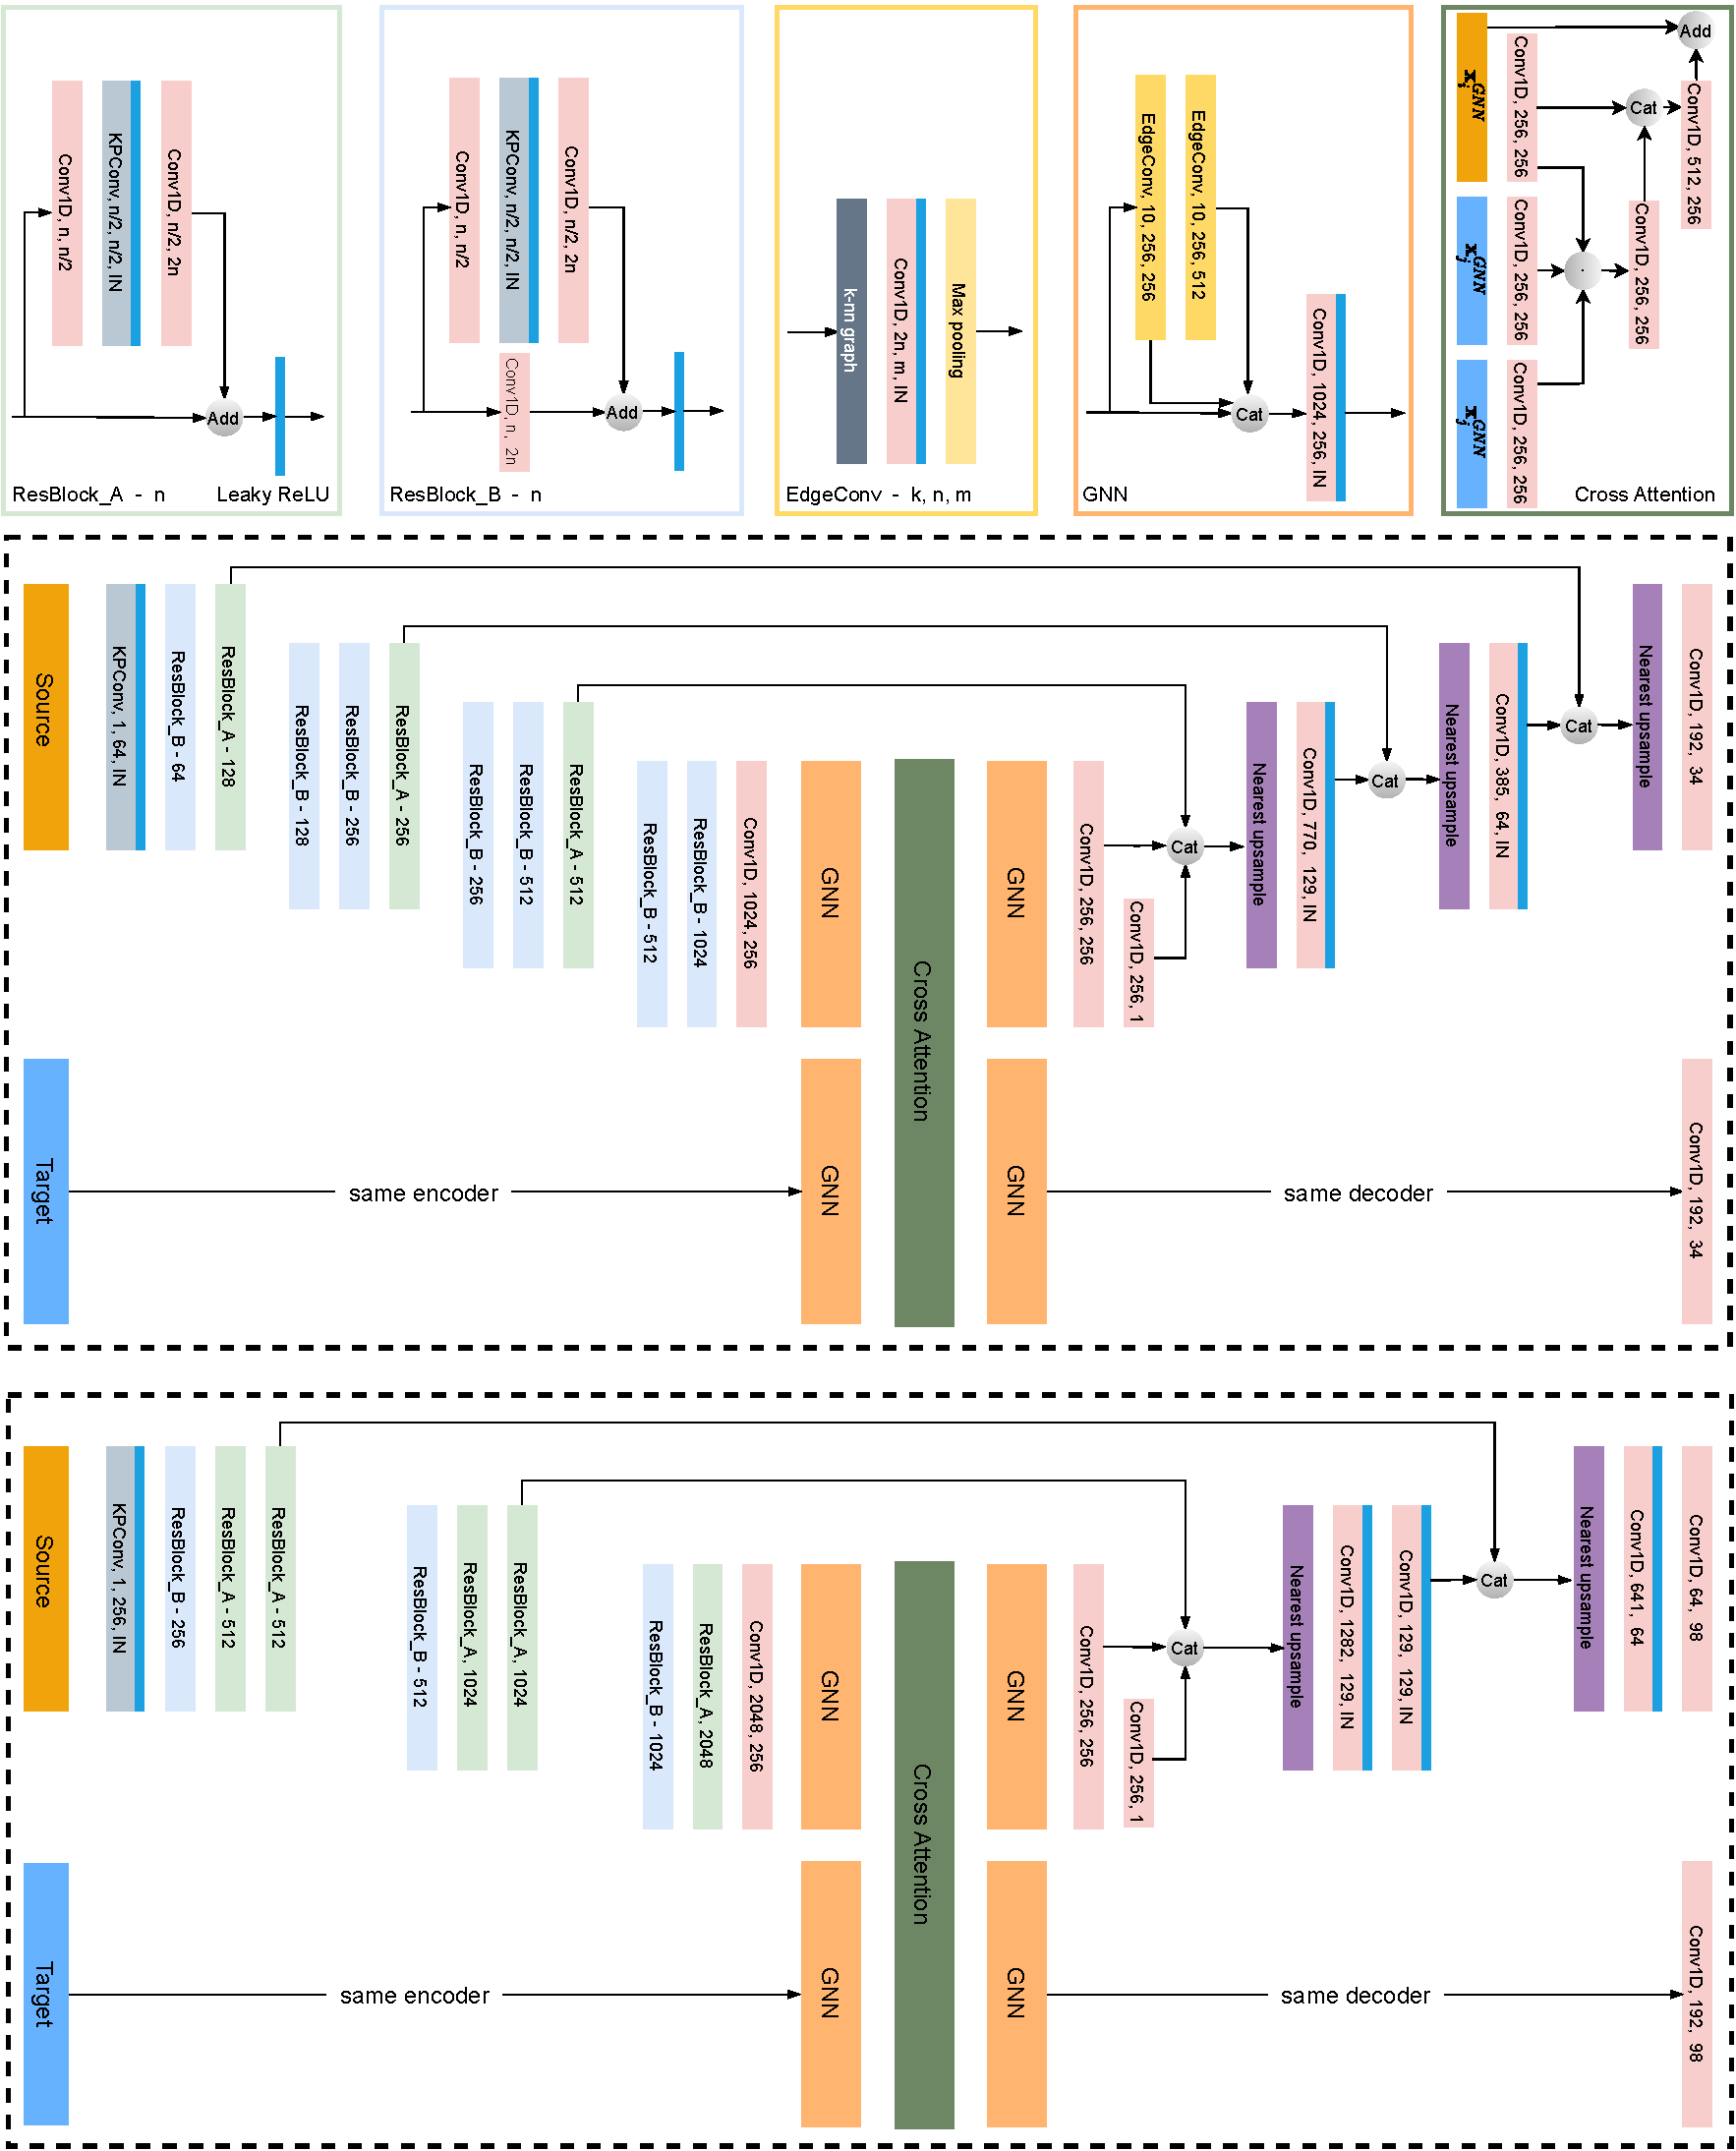
\includegraphics[width=0.95\textwidth]{figures/images/arch_sketch.pdf}
    \caption{Network architecture of \acro\ for \emph{3DMatch} (\textit{middle}) and \emph{ModelNet} (\textit{bottom}). In the cross attention module, for each (query $\mathbf{s}_i \in \mathbb{R}^{b\times1}$ , key $\mathbf{k}_i \in \mathbb{R}^{b\times1}$, value $\mathbf{v}_i \in \mathbb{R}^{b\times1}$), $\bigodot$ denotes first reshape them into shape $(4, \frac{b}{4})$(4 heads), then compute scores matrix $\mathbf{S}$ from $\mathbf{s}_i$ and $\mathbf{k}_i$, finally get message update from $\mathbf{v}_i$ and reshape back to $(b,1)$.}
    \label{fig:network_arch_detailed}
\end{figure}